% IEEE standard conference template; to be used with:
%   spconf.sty  - LaTeX style file, and
%   IEEEbib.bst - IEEE bibliography style file.
% --------------------------------------------------------------------------

\documentclass[letterpaper]{article}


\usepackage{spconf,amsmath,amssymb,graphicx}
\usepackage{ucs}
\usepackage[utf8x]{inputenc}
\usepackage[english]{babel}
\usepackage{calc}
\usepackage{enumitem}
\usepackage{listings}
\usepackage{xcolor}
\usepackage{url}

% Example definitions.
% --------------------
% nice symbols for real and complex numbers
\newcommand{\R}[0]{\mathbb{R}}
\newcommand{\C}[0]{\mathbb{C}}

% bold paragraph titles
\newcommand{\mypar}[1]{{\bf #1.}}

% monospace text
\makeatletter
\DeclareRobustCommand\ttfamily
        {\not@math@alphabet\ttfamily\mathtt
         \fontfamily\ttdefault\selectfont\hyphenchar\font=-1\relax}
\makeatother
\DeclareTextFontCommand{\mytexttt}{\ttfamily\hyphenchar\font=45\relax}

% Title.
% ------
\title{Escape Analysis for Multi-Threaded Javali}
%
% Single address.
% ---------------
\name{Andrei Pârvu, Sebastian Wicki}
\address{Department of Computer Science\\ ETH Z\"urich\\Z\"urich, Switzerland}



% For example:
% ------------
%\address{School\\
%    Department\\
%    Address}
%
% Two addresses (uncomment and modify for two-address case).
% ----------------------------------------------------------
% \twoauthors
 % {A. Andri Parvu, B. Sebastian Wicki}
  %    {ETH Zurich\\
  %    Department of Computer Science}
 % {C. Author-three, D. Author-four\sthanks{The fourth author performed the work
  %    while at ...}}
  %    {School C-D\\
  %    Department C-D\\
  %    Address C-D}


\begin{document}
%\ninept
%
\maketitle
%

\begin{abstract}
\textcolor{gray}{
Describe in concise words what you do, why you do it (not necessarily
in this order), and the main result.  The abstract has to be
self-contained and readable for a person in the general area. You
should write the abstract last. }
\end{abstract}

\section{Introduction}\label{sec:intro}

The basis of this project is an extended version of Javali with support for
basic multi-threading, similar to Java's built-in \texttt{Thread} class. 
Additionally, we also added support for synchronization though locks. Having
those additional language features also give more margin for potential
optimizations, which we will discuss in the following paragraphs.

\mypar{Motivation} \
Escape analysis can determine if an object reference escapes a certain dynamic
scope, for example the scope of a thread or the scope of a stack frame. This
information can be useful for a class of optimizations. In this project, we
explored two optimizations: Stack allocation of objects and synchronization
elision. Since Javali does not support modules or other forms of dynamic code
loading, we can perform a whole-program escape analysis, typically yielding more
precision.

In standard Javali, all non-primitive objects are allocated on the heap. The
existing implementation even leaks those objects, as there is currently on
garbage collection. Using escape analysis, the compiler can infer that certain
objects will never outlive the current stack frame, thus those objects could
be allocated on the stack. This has the advantage that the object will be cleaned
up automatically once the function returns. Additionally, allocating data on the
stack is typically faster than calling \texttt{malloc()} for heap allocation.
This is especially true in multi-threaded programs, as the implementation of
\texttt{malloc()} internally needs to synchronize as well, although modern
implementations such as \texttt{TCMalloc} \cite{TCMalloc} optimize this case heavily.

In this paper we provide an extended escape analysis for stack allocation that
even allows stack allocation for objects that are shared with other threads,
under the condition that the thread does not outlive the current function.
This is often the case in the fork-join programming model, where a function
forks multiple child threads to work on in parallel on some data, and then
waits for them to join.

As a second optimization, we implement synchronization removal on objects that
never escape the current thread, i.e. that are never shared among multiple threads
thus do not to be locked in order to be accessed safely. 

This optimization is useful for classes that are is written to be thread-safe,
i.e. use synchronization to ensure correctness, but are actually never used
in a multi-threaded setting, which leads to unnecessary overhead. Library
classes such as Java's \texttt{Vector} or \texttt{Hashtable} class are examples
of thread-safe library classes that were later replaced with non-synchronized
alternatives (namely \texttt{ArrayList} and \texttt{HashMap}) for better
performance.

\subsection{Related Work}

\mypar{Graph based approaches}
There exist numerous papers on escape analysis for Java. The most cited one,
which is also used by the Java HotSpot virtual machine \cite{HotSpot}, is the work by
Choi et al \cite{Choi:99}. They model the relationship of object in a so called
\emph{connection graph}, where objects are represented as nodes, and directed
edges represent the relationship among the objects. Nodes are marked with \emph{ArgEscape}
to indicate that they escape its method via arguments, \emph{GlobalEscape} is used
for nodes that could be accessed globally or by another thread, and \emph{NoEscape}
is used for nodes that do not escape.

A similar graph-based approach was published at the same time in the same journal
by Whaley and Rinard \cite{Whaley:99}. They also use a directed graph, called the points-to graph,
to represent objects. The escape information is determined by the type of edges
between objects: An object is said to escape its method when it is reachable via an outside edge.

Both approaches are flow-sensitive, they process the nodes of the control flow graph
individually and merge the resulting graphs where needed. Both approaches have a
intraprocedural phase where each method is processed individually, and a interprocedural
phase where the graphs are merged at call sites to yield more precise information.

A survey by King \cite{King:04} shows that the approach by Whaley and Rinard is more precise
than the algorithm by Choi et al, they are able to stack allocate more objects and
remove more synchronization.

\mypar{Alias Set based approaches}
A different approach for the purpose of lock removal is taken by Ruf \cite{Ruf:00}.
Every variable is associated with an alias set that represents all objects that
can be referenced by that variable. An alias set stores the alias sets of all
fields reachable by it, and whether the objects it represents are synchronized
or globally reachable. This approach also has separate intra- and interprocedural
phases, but it is flow-insensitive. In the survey by  King \cite{King:04} Ruf
yields the most precision of all algorithms for lock removal.

As Ruf's approach is only concerned about lock removal and works on a low-level
Java bytecode, his approach was generalized by Ranganath et al \cite{Ranganath:04}.
They extend alias sets to store more general thread escape information
and dependence information about Java source files.

For this project, we explored and extended two approaches: Stack escape analysis
is inspired by Whaley and Rinard, but does more effort to handle thread creation
and uses node labels similar to Choi.
% TODO Andrei, can you find more/better differences?

For lock removal we use an alias set based approach based on Ruf. However, we
use a more general notation of escaping objects similar to Ranganath et al. While
not implemented for this project, this would enable other optimizations such
as thread-local garbage collection. In our approach, alias sets are associated
with expressions instead of variables, to work with the Javali AST.

% TODO mention interprocedural phase?

\section{Background}\label{sec:background}

In this section we briefly present the programming interface and semantics of our
threading extension. In the second part, we formally introduce escape analysis.

\subsection{Threading and Synchronization in Javali}
The interface for multi-threading in Javali is heavily inspired by Java. In
order to create a new thread, the programmer has to create a new class that
inherits from the built-in \texttt{Thread} class and overwrite the \texttt{run()}
method to provide a thread entry point. 
The \texttt{Thread} class contains the following methods:

\begin{description}[leftmargin=!,labelwidth=\widthof{\texttt{start()}}]
 \item[\texttt{run()}] Thread entry point. To be overwritten by clients.
 \item[\texttt{start()}] Starts a new thread. Like in Java it is an error to
 call this method more than once on the same receiver.
 \item[\texttt{join()}] Blocks the caller until the thread exits. It is an error
 to call this on a thread that was never started or was already joined.
\end{description}

Similar to Java, our extension to Javali has a built-in lock and conditional variable
within every object. A notable difference to Java however is that there is
no special syntax for locking, the built-in \texttt{Object} just provides the
following methods.

\begin{description}[leftmargin=!,labelwidth=\widthof{\texttt{unlock()}}]
 \item[\texttt{lock()}] Locks the receiver object. If the object was already locked by
 another thread, the current thread is blocked until the object is unlocked. The
 lock is re-entrant in the sense that a thread can call this method on objects
 on which it already own the lock.
 \item[\texttt{unlock()}] Unlocks the object. Also re-entrant in the sense that
 in order to fully unlock an object,
 the lock owner needs to call \texttt{unlock()} as many times as \texttt{lock()}
 was called. It is an error to call \texttt{unlock()} without owning the lock.
 \item[\texttt{wait()}] Causes the calling thread to wait until another thread
 calls \texttt{notify()} on the object.
 \item[\texttt{notify()}] Wakes up another thread waiting on this object.
\end{description} % TODO double check notify/wait semantics

\subsection{Escape Analysis}

The purpose of escape analysis is to determine whether an object escapes a certain
scope, in our case whether it escapes a certain method and its stack or a certain thread.

\mypar{Stack Escaping} For stack allocation we needed to implement an algorithm which can determine
if a certain variable (or field) escapes the method in which it is allocated. If the object does not
escape, then it can be allocated on the stack. Otherwise, we must distinguish between other cases:
\begin{itemize}
  \item the object is referenced by a parameter - in this case it might be allocated on the stack
  of the caller (TODO: we currently don't do this in the code)
  \item the object is returned - then it might either be allocated on the stack of the caller of freed
  by the caller
  \item the object is referenced by \textit{this}
  \item the object is passed to another thread
\end{itemize}
In order to achieve these goals we decided to implement and expand the escape-analysis algorithm presented
in \cite{Whaley:99}.

\mypar{Thread Escaping} In order to safely remove locks, the receiver object must
not be locked in other threads. In our analysis, we therefore remove locks only
if an object is never reachable from another thread  An object is said to
escape a thread if:

\begin{itemize}
  \item it inherits from the \textit{Thread} class and \texttt{.start()} is called on that object.
  \item the object is (transitively) reachable from a field of another escaped object.
\end{itemize}

\section{Proposed Method}\label{sec:yourmethod}

In this section we present our algorithms used in escape analysis.
The \emph{points-to escape graph} determines to whether an object can
be allocated on the stack, the \emph{alias sets} inform us whether we can
safely remove invocations of \texttt{.lock()} and \texttt{.unlock()}.

\subsection{Points-To Escape Graph}
The algorithm shown in \cite{Whaley:99} constructs, for each method,
a graph in which nodes represent allocated objects and edges represent references between objects.
The nodes with in-degree zero are either locally declared variables, method parameters, or the \textit{this}
object. Edge between nodes can either be labeled with the name of a field, or ... TODO. As described in
section \ref{sec:background}, each node can have one of the following labels: REF\_PARAM, THREAD, ARRAY, THIS and ESCAPED. \\
An example program is shown in Listing~\ref{lst:program}. with the associated escape-graph shown in Figure~\ref{fig:escapegraph}.
One can observe that the nodes have been classified as following:
\begin{itemize}
  \item Node 5, corresponding to t.arg has labels THREAD and REF\_PARAM, because t is a parameter and also a thread object.
  \item Node 4, corresponding to e has only label REF\_PARAM
  \item Node 14 and 1 have the THIS label
\end{itemize}
% TODO having no special syntax is not that bad without exceptions


\lstset{language=Java,
           basicstyle=\ttfamily\scriptsize,
          breaklines=true
          }
\begin{lstlisting}[caption=Example program, label=lst:program]
class Custom extends Thread {
    Box arg;
    void run() {
        write(arg.val); writeln();
    }
}

class Box {
    int val;
}

class Main {
    Box b;
    void escapeOne(Custom t, Box e) {
        write(b.val); writeln();
        t.arg = e;
        t.start();

        t.join();
    }

    void main() {
        Custom t;
        Box b, e;

        b = new Box();
        e = new Box();
        b.val = 23;
        e.val = 42;

        this.b = b;

        t = new Custom();
        escapeOne(t, e);
     }
}
\end{lstlisting}

\begin{figure} \center
 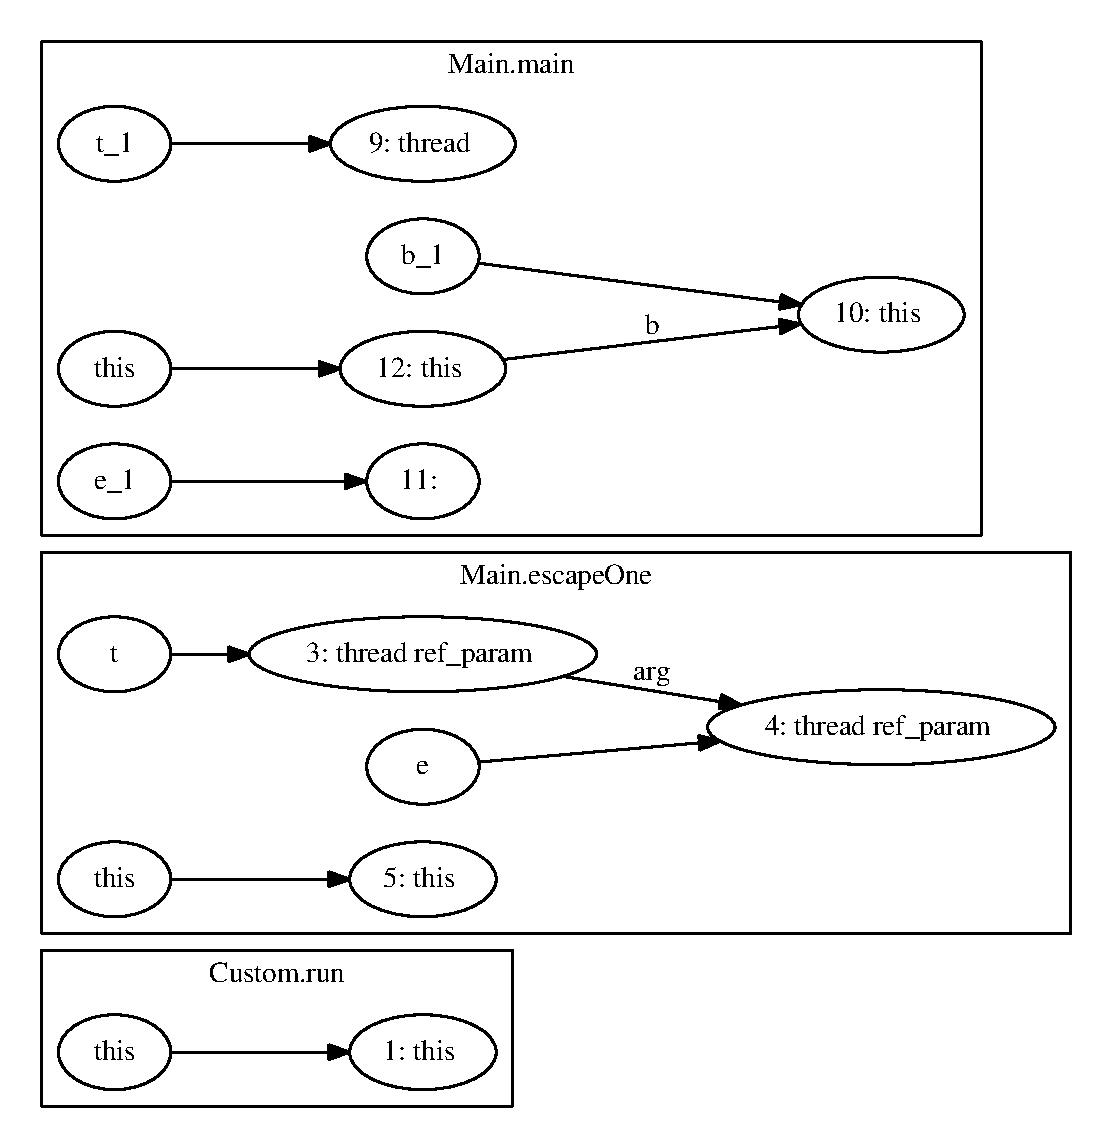
\includegraphics[width=0.8\linewidth]{EscapeTest.eps}
  \caption{Points-to-escape graph}
  \label{fig:escapegraph}
\end{figure}

\mypar{Building the graph for a method}. The escape graph is built in an iterative manner using control-flow analysis.
First of all each basic block is processed, in a bread-first search manner, and all its instructions are added to a
basic-block local escape-graph.
Secondly, the escape graph of each basic block is merged with the escape graphs of its predecessors and the process
is repeated until no more changes occur. Finally, after the graph is completed, a depth-first search is applied on it,
in order to spread the labels of the nodes to the set of nodes it references.

\mypar{Analyzing a method call}. The first approach we had to analyzing method calls was to map the parameters of the given
call to the corresponding nodes in the escape graph of the callee and copy the already computed labels from the callee to the
caller. Unfortunately, this solution misses cases in which different fields of parameters are assigned to each other in the callee
(one example is shown in Listing~\ref{lst:fields}). In order to address this problem we decided to recurse into the callee and
construct it's escape graph given the parameter nodes of the caller. Although this increases the overall complexity of our solution,
it provides a more accurate analysis.

\begin{lstlisting}[caption=Field parameter assignment, label=lst:fields]
void main() {
  F f1, f2;

  f1 = new F();
  f1.next = new F();

  f2 = new F();
  f2.next = new F();

  d1(f1, f2);

  this.f = f1;
}

void d1(F f1, F f2) {
  f1.next = f2.next;
}
\end{lstlisting}

\mypar{Analyzing thread objects}. One special case of escaping variables are threads. We defined a thread object to escape if
it the thread was started, but I was not joined later on in the method (TODO: maybe find a better sentence).
Therefore, in order to determine if the \textit{join} method was called on every possible path from the starting point
to the \textit{end} basic block we need to do another control-flow analysis. For every basic block in the method we 
determine the set of thread objects that have \textit{join} calls on every path from that basic block to the end (let's call this set \textit{join\_set}).
If we have a \textit{start} call-site for a certain thread object and that object is not in the \textit{join\_set} of that
method, then the object escapes.
It should be mentioned that currently we only to this analysis for variable objects (not for fields) and we do not do any inter-procedural analysis for thread objects.

\subsection{Alias Sets}

To infer whether an object is shared among multiple threads, we associate \emph{alias sets}
with every expression in the Javali AST. We use the same notation as introduced by Ruf \cite{Ruf:00}.
An alias set summarizes the information about all abstract objects that are the result of the expression, it is defined as follows:

\begin{equation*}
\begin{split}
    aliasSet &::= \bot \mid \langle escapes, fieldMap \rangle \\
    aliasContext &::= \langle this, \langle a_{1}, a_{2}, a_{3},~\dots \rangle, result \rangle
\end{split}
\end{equation*}

$\bot$ denotes an expression of a primitive type, it does not contain any other information.

$escapes$ is a boolean which is \emph{true} if the objects represented by the alias set escape its thread.

$fieldMap$ associates every field $f$ of the abstract object with an alias set which represents the objects stored in field $f$.
The special field \texttt{\$ELT} denotes the elements of an array.

Alias sets can be \emph{unified}. This operation merges the information of two alias sets and creates a new, unified alias set.
If an object in one of the two alias set $escapes$, the object will escape in the resulting alias set as well.

In order to propagate information at method boundaries, the concept of \emph{alias contexts} is introduced, they
are n-tuples of alias sets associated with a method, representing the alias sets of the methods signature.

We differentiate between alias contexts associated with formal method symbols, the \emph{method contexts} and the
alias contexts that store information about method calls at call sites, the \emph{site contexts}.

\mypar{Intraprocedural analysis} After creating the call graph and partitioning it 
into strongly connected components using Tarjan's algorithm, the analysis processes all methods,
traversing the call graph bottom-up. The goal of this first phase is to populate the
method contexts. Because the callees are analyzed before the callers, the method
contexts will tell us if an objected passed as an argument will escape to other threads.

The rules for processing a methods statements are based on Ruf's \cite{Ruf:00} paper. Alias sets are merged
at assignments, field and array access create new entries in the $fieldMap$ attribute. 
For each method invocation, an \emph{site context} is created and then unified with
a clone of the method context of all callees. For methods belonging to the same strongly connected component, i.e.
methods that call each other recursively, the method context of the callees are modified during unification.

If the target of a method call is \texttt{Thread.start()}, we mark the receiver object and all reachable fields
in the callees site context and the threads entry method as escaped.
In order to not eliminate locks around \texttt{notify()} and \texttt{wait()}, we also mark those receiver
object as escaping. 

\mypar{Interprocedural analysis}
The purpose of the second phase is to push down information about escaped objects from callers to callees.
For this reason, it traverses the call graph top-down. Some calls to a specific method might call it
with escaped objects, other calls might not. When we merge clones of the site and method contexts,
this fact will be reflected in the unified method context. 

For this reason, we tried to store and deduplicate those alias contexts, and use them as a method context
for visiting the callees. This would allow us to create specialized methods based on the different
method context created in this phase. However, we were not able to correctly implement this phase in time,
so the current code naivly merges all site contexts with the single method context of a method.

We store the alias sets inline the AST, so the thread escape information is available for the code
generator.

The final method context summaries generated for the example in Listing~\ref{lst:program} looks as follows:

{ \footnotesize

\begin{description}
\item[\texttt{Main.main()}] \hfill \\
    $ this: \langle false, \{ b:\langle false, \{ \} \rangle\} \rangle $ \\ 
    $ arguments: \lbrack \rbrack $ \\
    $ result: \bot  $ 
\item[\texttt{Main.escapeOne()}] \hfill \\
    $ this: \langle false, \{ b:\langle false, \{ \} \rangle\} \rangle $ \\
    $ arguments: \lbrack \langle true, \{ arg:\langle true, \{ \} \rangle\} \rangle, \langle true, \{ \} \rangle \rbrack $ \\
    $ result: \bot $
\item[\texttt{Custom.run()}] \hfill \\
 $ this: \langle true, \{ arg:\langle true, \{ \} \rangle\} \rangle $ \\
 $ arguments: \lbrack \rbrack $ \\ 
 $ result: \bot $
\end{description}
}

Both, the created thread as well as the argument passed to it are marked as escaped. The \texttt{Main} object however
has $escapes$ set to $false$.

\mypar{Code Generation}
As stated above, we were not able to implement method specialization in time. The code generation
therefore looks at the receiver alias set of a \texttt{.lock()} or  \texttt{.unlock()} method
call and omits the function call. As the receiver expression might contain side effects, it
is still generated.

Additionally, for objects which never escape its thread, we omit calling the object initialization
function which sets up the built-in lock and conditional variable.


\section{Experimental Results}\label{sec:exp}


\mypar{Experimental setup} For the experiments we used two different machines. The first one, running
Ubuntu 14.04 with a i5-3317U, 1.70GHz processor and 4Gb RAM.

We tried to analyze three different aspects of our project: firstly, the running time improvement of just allocating
the unescaped objects on the stack. Secondly, we wanted to see the time benefit of working with stack-allocated
objects instead of heap-allocated ones. And thirdly, we tried to observe the how lock-removal affects single-threaded
programs.\\

\mypar{Results}
For the first experiment, we just allocated various objects without using them afterwards, in order to see how the running time differs
for both cases. The results can be seen in Figure~\ref{fig:alloc}TODO: comment on the results\\

In the second experiment, we wrote a basic matrix multiplication program with the intent of observing how execution time changes when using
stack allocation. The results can be seen in Figure~\ref{fig:matrixmul}. It can be observed that the stack allocation improves running
time with almost 20\%, with the obvious draw-back that more stack memory is used.\\

For the third experiment, we implemented a hash map, which simulates string hashing (because Javali doesn't have strings we used ASCII arrays).
The hash map is implemented to be thread-safe, so we ran the experiment with one thread and lock removal. Results can be seen in Figure~
\ref{fig:hash}; with lock removal, running time is approximately 10\% faster than the unanalyzed version.\\

\begin{figure} \center
 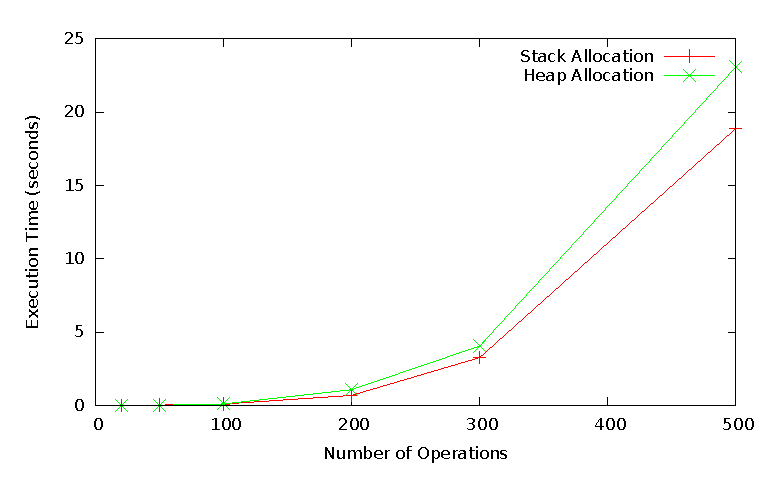
\includegraphics[width=0.8\linewidth]{results_matrix_mul.eps}
  \caption{Running times matrix multiplication}
  \label{fig:matrixmul}
\end{figure}

\begin{figure} \center
 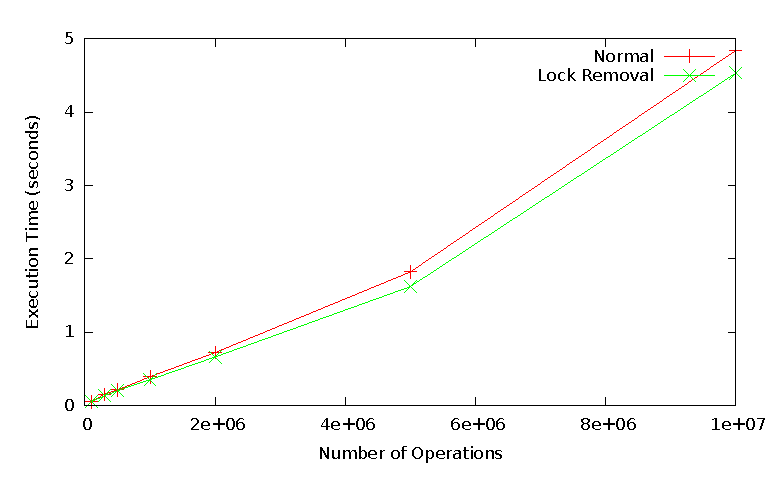
\includegraphics[width=0.8\linewidth]{results_hash.eps}
  \caption{Running times hash map}
  \label{fig:hash}
\end{figure}

\begin{figure} \center
 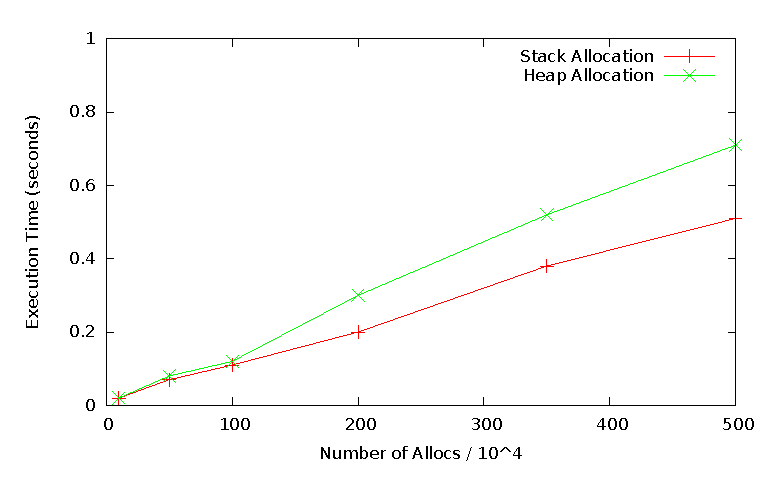
\includegraphics[width=0.8\linewidth]{results_only_alloc.eps}
  \caption{Running times only alloc}
  \label{fig:alloc}
\end{figure}

\begin{figure} \center
 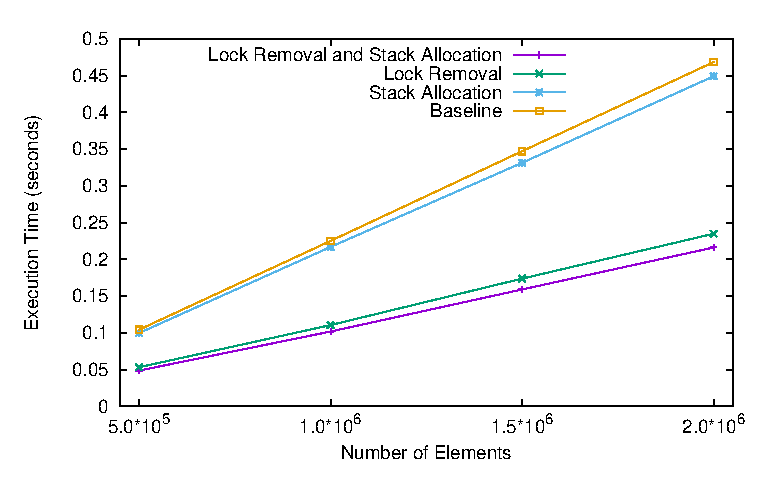
\includegraphics[width=0.8\linewidth]{results_merge.eps}
  \caption{Running times for parallel merge sort}
  \label{fig:merge}
\end{figure}

\section{Conclusions}

\textcolor{gray}{
Here you need to summarize what you did and why this is
important. {\em Do not take the abstract} and put it in the past
tense. Remember, now the reader has (hopefully) read the report, so it
is a very different situation from the abstract. Try to highlight
important results and say the things you really want to get across
such as high-level statements (e.g., we believe that .... is the right
approach to .... Even though we only considered x, the
.... technique should be applicable ....) You can also formulate next
steps if you want. Be brief. After the conclusions there are only the references.
}

% References should be produced using the bibtex program from suitable
% BiBTeX files (here: bibl_conf). The IEEEbib.bst bibliography
% style file from IEEE produces unsorted bibliography list.
% -------------------------------------------------------------------------
\bibliographystyle{IEEEbib}
\bibliography{report}

\end{document}
